%% Requires compilation with XeLaTeX or LuaLaTeX
\documentclass[10pt,xcolor={table,dvipsnames},t]{beamer}
\usetheme{UCBerkeley}

\title[\LaTeX]{\LaTeX}
\subtitle{Info 98: Practical Data Science Skills for Internships}
\author{Data Science Society at Berkeley}
\institute{datasciencedecal@gmail.com}
\date{September 10th, 2018}

\begin{document}

\begin{frame}
  \titlepage
\end{frame}

% Uncomment these lines for an automatically generated outline.
%\begin{frame}{Outline}
%  \tableofcontents
%\end{frame}

\section{Introduction}
 
 \begin{frame}
\frametitle{First, some important logistical stuff}
1.) Check to see that you are on bCourses. This is \textit{critical.} The syllabus should be on there as well.\\\\
2.) Join our Piazza using this link:\\\\
\begin{center}
https://piazza.com/berkeley/fall2018/info98 \\\\
\end{center}
\textbf{Attendance policy}: You must submit a code to bCourses every lecture to "prove" that you attended. The code will be written on the board at some point during class.\\

\end{frame}

\begin{frame}{Why \LaTeX ?}

\begin{block}{Disclaimer:}

\LaTeX \ is actually not a critical skill for data science

\end{block}

\begin{block}{So why the hell are we teaching this?}
\begin{itemize}
\item It requires no prior coding experience.
\item For the purposes of this course, we needed a coding language that everyone could use for the collaborative git project.
\item It is very useful for writing papers that involve math or code.
\item It can be used to display math elegantly in Jupyter notebooks.
\item \ \  \ \ \ \ \ \ \ \ \textit{This presentation was written entirely in \LaTeX}

\end{itemize}
\end{block}
\end{frame}
 
\begin{frame}
\frametitle{Introduction to Overleaf}
\LaTeX is actually quite annoying to learn on your own if you are used to just using Google Docs or Microsoft Word.\\~\\

For the purposes of this demonstration, we will be easing you into the process by introducing you to the \textbf{Overleaf editor} and, later on, showing off some really cool templates. \\\\\\
You can follow along this presentation using this link:\\\\
\begin{center}
https://v2.overleaf.com/read/zthjmxpnhpvp
\end{center}
\end{frame}
 
\section{Some \LaTeX{} Examples}

\subsection{Mathematics}

\begin{frame}{Readable Mathematics}

Let $X_1, X_2, \ldots, X_n$ be a sequence of independent and identically distributed random variables with $\text{E}[X_i] = \mu$ and $\text{Var}[X_i] = \sigma^2 < \infty$, and let
$$S_n = \frac{X_1 + X_2 + \cdots + X_n}{n}
      = \frac{1}{n}\sum_{i}^{n} X_i$$
denote their mean. Then as $n$ approaches infinity, the random variables $\sqrt{n}(S_n - \mu)$ converge in distribution to a normal $\mathcal{N}(0, \sigma^2)$.

\end{frame}


\subsection{Tables and Figures}

\smallframetitle

\begin{frame}{Tables and Figures}

\begin{itemize}
\item Use \texttt{tabular} for basic tables --- see Table~\ref{tab:widgets}, for example.
\item You can upload a figure (JPEG, PNG or PDF) using the files menu. 
\item To include it in your document, use the \texttt{includegraphics} command (see the comment below in the source code).
\end{itemize}

\begin{table}
\centering
\begin{tabular}{l r}
\tableheadrow
\tableheadcol{Item} & \tableheadcol{Quantity} \\
Widgets & 42 \\
Gadgets & 13
\end{tabular}
\caption{\label{tab:widgets}An example table.}
\end{table}

\end{frame}

\begin{frame}
\frametitle{Incorporating figures and pictures}

This is the three way Venn diagram for "Computer Science using Big Data," "Math and Statistics,"

\begin{figure}
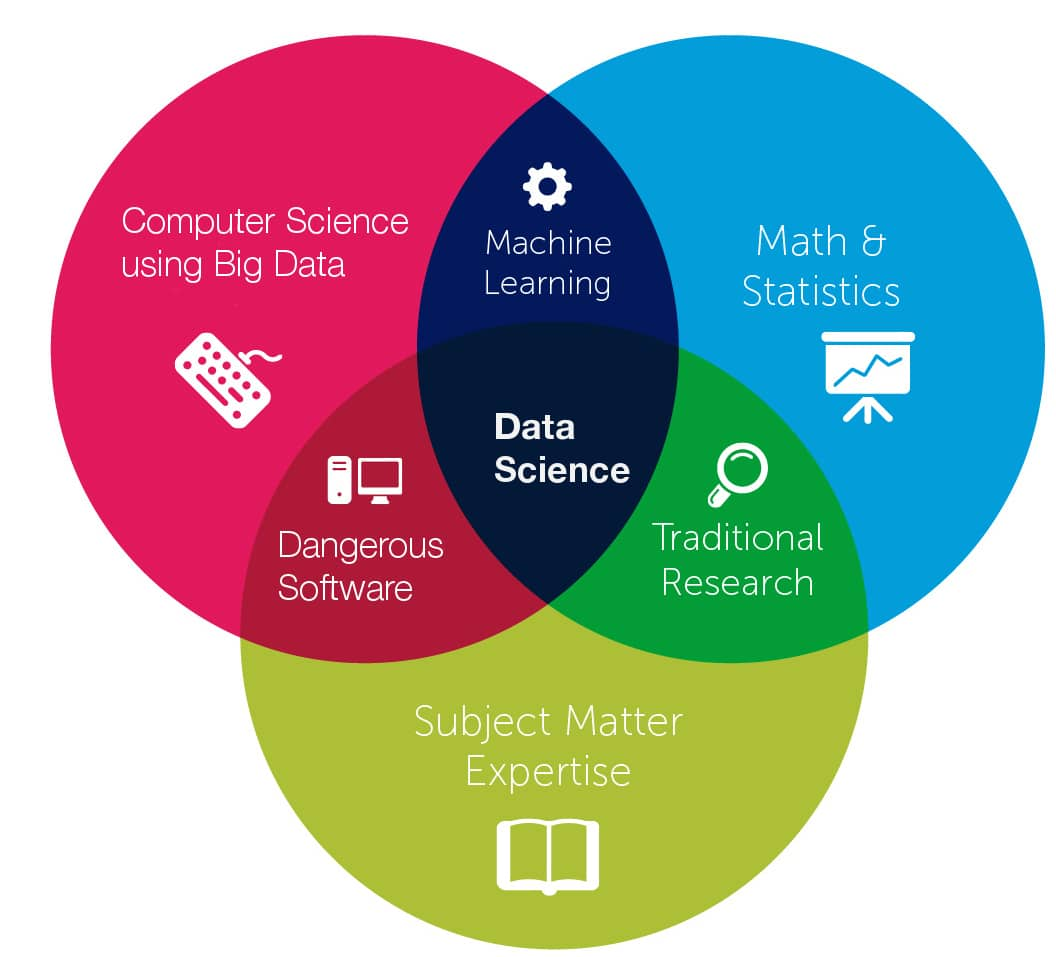
\includegraphics[width=.45\textwidth,height=.45\textheight]{datascience}
\caption{\label{fig:your-figure}Data Science = CS + Math and Stats + Subject Matter Expertise.}
\end{figure}
\end{frame}


\begin{frame}
\frametitle{Multiple columns}

\begin{columns}[T]

\begin{column}{0.48\textwidth}
\small
\LaTeX \ can feel extremely clunky at times. \newline 
But, if you know how to use it, it is extremely versatile.
\end{column}

\begin{column}{0.48\textwidth}
\begin{itemize}
\item First bullet goes here
  \begin{itemize}
  \item Secondary bullet goes here
    \begin{itemize}
    \item Tertiary bullet goes here
    \end{itemize}
  \end{itemize}
\end{itemize}
\end{column}

\end{columns}
\end{frame}

\begin{frame}
\frametitle{Theorem}
\begin{theorem}["Best" Linear Predictor for 2 Variables]
\begin{center} 
L(Y|X) = E[Y] + $\frac{cov(X,Y)}{var(X)}[X-E[X]]$
\end{center}
\end{theorem}
\end{frame}

\begin{frame}[fragile] % Need to use the fragile option when verbatim is used in the slide
\frametitle{Verbatim}
\begin{example}[Code for Previous Slide]
\begin{verbatim}
\begin{frame}
\frametitle{Theorem}
\begin{theorem}["Best" Linear Predictor for 2 Variables]
\begin{center} 
L(Y|X) = E[Y] + $\frac{cov(X,Y)}{var(X)}[X-E[X]]$
\end{center}
\end{theorem}
\end{frame}\end{verbatim}
\end{example}
\end{frame}



\begin{frame}
\Huge{INTERACTIVE DEMO TIME :D}
\end{frame}

\begin{frame}
\frametitle{Next Two Assignments}
\begin{block}{Update Your R\'esum\'e}
This is a \textit{solo assignment} due \underline{9/16/18 11:59 PM}. You \textbf{must} use \LaTeX \ to create your r\'esum\'e.
\end{block}

\begin{block}{Design a DeCal Syllabus}
This is a \textit{group assignment} due \underline{9/30/18 11:59 PM}. Groups can only be in sizes of \textbf{\underline{3 or 4}}.\newline
\end{block} $Rubrics\ for\ both\ of\ these\ assignments\ can\ be\ found\ on\ the\ syllabus.$
\end{frame}

\begin{frame}
\frametitle{Additional Resources}
\begin{itemize}
\item https://en.wikibooks.org/wiki/LaTeX/
\newline
\item https://tex.stackexchange.com
\newline
\item https://www.latex-tutorial.com/tutorials/
\newline
\item https://texblog.org
\newline
\item https://www.sharelatex.com/learn
\end{itemize}
\end{frame}


\end{document}
